\documentclass[twoside]{book}

% Packages required by doxygen
\usepackage{fixltx2e}
\usepackage{calc}
\usepackage{doxygen}
\usepackage[export]{adjustbox} % also loads graphicx
\usepackage{graphicx}
\usepackage[utf8]{inputenc}
\usepackage{makeidx}
\usepackage{multicol}
\usepackage{multirow}
\PassOptionsToPackage{warn}{textcomp}
\usepackage{textcomp}
\usepackage[nointegrals]{wasysym}
\usepackage[table]{xcolor}

% Font selection
\usepackage[T1]{fontenc}
\usepackage[scaled=.90]{helvet}
\usepackage{courier}
\usepackage{amssymb}
\usepackage{sectsty}
\renewcommand{\familydefault}{\sfdefault}
\allsectionsfont{%
  \fontseries{bc}\selectfont%
  \color{darkgray}%
}
\renewcommand{\DoxyLabelFont}{%
  \fontseries{bc}\selectfont%
  \color{darkgray}%
}
\newcommand{\+}{\discretionary{\mbox{\scriptsize$\hookleftarrow$}}{}{}}

% Page & text layout
\usepackage{geometry}
\geometry{%
  a4paper,%
  top=2.5cm,%
  bottom=2.5cm,%
  left=2.5cm,%
  right=2.5cm%
}
\tolerance=750
\hfuzz=15pt
\hbadness=750
\setlength{\emergencystretch}{15pt}
\setlength{\parindent}{0cm}
\setlength{\parskip}{3ex plus 2ex minus 2ex}
\makeatletter
\renewcommand{\paragraph}{%
  \@startsection{paragraph}{4}{0ex}{-1.0ex}{1.0ex}{%
    \normalfont\normalsize\bfseries\SS@parafont%
  }%
}
\renewcommand{\subparagraph}{%
  \@startsection{subparagraph}{5}{0ex}{-1.0ex}{1.0ex}{%
    \normalfont\normalsize\bfseries\SS@subparafont%
  }%
}
\makeatother

% Headers & footers
\usepackage{fancyhdr}
\pagestyle{fancyplain}
\fancyhead[LE]{\fancyplain{}{\bfseries\thepage}}
\fancyhead[CE]{\fancyplain{}{}}
\fancyhead[RE]{\fancyplain{}{\bfseries\leftmark}}
\fancyhead[LO]{\fancyplain{}{\bfseries\rightmark}}
\fancyhead[CO]{\fancyplain{}{}}
\fancyhead[RO]{\fancyplain{}{\bfseries\thepage}}
\fancyfoot[LE]{\fancyplain{}{}}
\fancyfoot[CE]{\fancyplain{}{}}
\fancyfoot[RE]{\fancyplain{}{\bfseries\scriptsize Generated by Doxygen }}
\fancyfoot[LO]{\fancyplain{}{\bfseries\scriptsize Generated by Doxygen }}
\fancyfoot[CO]{\fancyplain{}{}}
\fancyfoot[RO]{\fancyplain{}{}}
\renewcommand{\footrulewidth}{0.4pt}
\renewcommand{\chaptermark}[1]{%
  \markboth{#1}{}%
}
\renewcommand{\sectionmark}[1]{%
  \markright{\thesection\ #1}%
}

% Indices & bibliography
\usepackage{natbib}
\usepackage[titles]{tocloft}
\setcounter{tocdepth}{3}
\setcounter{secnumdepth}{5}
\makeindex

% Hyperlinks (required, but should be loaded last)
\usepackage{ifpdf}
\ifpdf
  \usepackage[pdftex,pagebackref=true]{hyperref}
\else
  \usepackage[ps2pdf,pagebackref=true]{hyperref}
\fi
\hypersetup{%
  colorlinks=true,%
  linkcolor=blue,%
  citecolor=blue,%
  unicode%
}

% Custom commands
\newcommand{\clearemptydoublepage}{%
  \newpage{\pagestyle{empty}\cleardoublepage}%
}

\usepackage{caption}
\captionsetup{labelsep=space,justification=centering,font={bf},singlelinecheck=off,skip=4pt,position=top}

%===== C O N T E N T S =====

\begin{document}

% Titlepage & ToC
\hypersetup{pageanchor=false,
             bookmarksnumbered=true,
             pdfencoding=unicode
            }
\pagenumbering{alph}
\begin{titlepage}
\vspace*{7cm}
\begin{center}%
{\Large My Project }\\
\vspace*{1cm}
{\large Generated by Doxygen 1.8.12}\\
\end{center}
\end{titlepage}
\clearemptydoublepage
\pagenumbering{roman}
\tableofcontents
\clearemptydoublepage
\pagenumbering{arabic}
\hypersetup{pageanchor=true}

%--- Begin generated contents ---
\chapter{Hierarchical Index}
\section{Class Hierarchy}
This inheritance list is sorted roughly, but not completely, alphabetically\+:\begin{DoxyCompactList}
\item \contentsline{section}{Camera}{\pageref{class_camera}}{}
\item \contentsline{section}{Dvector}{\pageref{class_dvector}}{}
\item \contentsline{section}{Gerstner\+Wave}{\pageref{class_gerstner_wave}}{}
\item \contentsline{section}{Height}{\pageref{class_height}}{}
\item \contentsline{section}{Ocean}{\pageref{class_ocean}}{}
\item \contentsline{section}{Wave\+Model}{\pageref{class_wave_model}}{}
\begin{DoxyCompactList}
\item \contentsline{section}{Gerstner\+Wave\+Model}{\pageref{class_gerstner_wave_model}}{}
\item \contentsline{section}{Philips\+Wave\+Model}{\pageref{class_philips_wave_model}}{}
\end{DoxyCompactList}
\end{DoxyCompactList}

\chapter{Class Index}
\section{Class List}
Here are the classes, structs, unions and interfaces with brief descriptions\+:\begin{DoxyCompactList}
\item\contentsline{section}{\hyperlink{class_camera}{Camera} }{\pageref{class_camera}}{}
\item\contentsline{section}{\hyperlink{class_dvector}{Dvector} \\*Classe representant un vecteur de double }{\pageref{class_dvector}}{}
\item\contentsline{section}{\hyperlink{class_gerstner_wave}{Gerstner\+Wave} \\*Classe representant une onde de Gerstner }{\pageref{class_gerstner_wave}}{}
\item\contentsline{section}{\hyperlink{class_gerstner_wave_model}{Gerstner\+Wave\+Model} \\*Modèle de Gerstner }{\pageref{class_gerstner_wave_model}}{}
\item\contentsline{section}{\hyperlink{class_height}{Height} \\*Classe representant un tableau 2D de double }{\pageref{class_height}}{}
\item\contentsline{section}{\hyperlink{class_ocean}{Ocean} \\*Classe faisant la synthèse de toutes les données -\/ calculs des hauteurs }{\pageref{class_ocean}}{}
\item\contentsline{section}{\hyperlink{class_philips_wave_model}{Philips\+Wave\+Model} }{\pageref{class_philips_wave_model}}{}
\item\contentsline{section}{\hyperlink{class_wave_model}{Wave\+Model} }{\pageref{class_wave_model}}{}
\end{DoxyCompactList}

\chapter{File Index}
\section{File List}
Here is a list of all documented files with brief descriptions\+:\begin{DoxyCompactList}
\item\contentsline{section}{{\bfseries camera.\+hxx} }{\pageref{camera_8hxx}}{}
\item\contentsline{section}{\hyperlink{_dvector_8h}{Dvector.\+h} \\*Vecteur de base (T\+P1 et T\+P2) }{\pageref{_dvector_8h}}{}
\item\contentsline{section}{{\bfseries F\+F\+T.\+h} }{\pageref{_f_f_t_8h}}{}
\item\contentsline{section}{{\bfseries Gerstner\+Wave.\+h} }{\pageref{_gerstner_wave_8h}}{}
\item\contentsline{section}{{\bfseries Gerstner\+Wave\+Model.\+h} }{\pageref{_gerstner_wave_model_8h}}{}
\item\contentsline{section}{{\bfseries gl\+\_\+defs.\+hxx} }{\pageref{gl__defs_8hxx}}{}
\item\contentsline{section}{{\bfseries Height.\+h} }{\pageref{_height_8h}}{}
\item\contentsline{section}{{\bfseries Ocean.\+h} }{\pageref{_ocean_8h}}{}
\item\contentsline{section}{{\bfseries Philips\+Wave\+Model.\+h} }{\pageref{_philips_wave_model_8h}}{}
\item\contentsline{section}{{\bfseries Wave\+Model.\+h} }{\pageref{_wave_model_8h}}{}
\item\contentsline{section}{{\bfseries window.\+hxx} }{\pageref{window_8hxx}}{}
\end{DoxyCompactList}

\chapter{Class Documentation}
\hypertarget{class_camera}{}\section{Camera Class Reference}
\label{class_camera}\index{Camera@{Camera}}


{\ttfamily \#include $<$camera.\+hxx$>$}

\subsection*{Public Types}
\begin{DoxyCompactItemize}
\item 
enum \hyperlink{class_camera_a3ba12bb77fc0e6ce7048a7c03c7fa776}{K\+E\+Y\+B\+O\+A\+RD} \{ {\bfseries A\+Z\+E\+R\+TY}, 
{\bfseries Q\+W\+E\+R\+TY}
 \}
\end{DoxyCompactItemize}
\subsection*{Public Member Functions}
\begin{DoxyCompactItemize}
\item 
\hyperlink{class_camera_a09942dcf1bbcf89bbca39601b9f273be}{Camera} (\hyperlink{class_camera_a3ba12bb77fc0e6ce7048a7c03c7fa776}{K\+E\+Y\+B\+O\+A\+RD}, float, float, float, float, float, float, float, int, int)
\item 
\hypertarget{class_camera_a7bc94fe5b01cd16da44630bd64ec741f}{}\label{class_camera_a7bc94fe5b01cd16da44630bd64ec741f} 
int {\bfseries get\+MouseX} ()
\item 
\hypertarget{class_camera_a9f384f3c203241bf4008211a4664722f}{}\label{class_camera_a9f384f3c203241bf4008211a4664722f} 
int {\bfseries get\+MouseY} ()
\item 
\hypertarget{class_camera_a67b651e8e6e82483ac5b6bad6521412c}{}\label{class_camera_a67b651e8e6e82483ac5b6bad6521412c} 
float {\bfseries get\+SightX} ()
\item 
\hypertarget{class_camera_a1e460da4c97d1ea672263352fb643af4}{}\label{class_camera_a1e460da4c97d1ea672263352fb643af4} 
float {\bfseries get\+SightY} ()
\item 
\hypertarget{class_camera_af99fd2297879cac1096d890c037cc6ea}{}\label{class_camera_af99fd2297879cac1096d890c037cc6ea} 
float {\bfseries get\+SightZ} ()
\item 
\hypertarget{class_camera_ae7c46d026313f6faefdcfdb5094ea8cb}{}\label{class_camera_ae7c46d026313f6faefdcfdb5094ea8cb} 
float {\bfseries getX} ()
\item 
\hypertarget{class_camera_ad71d83315248602503546eba37697390}{}\label{class_camera_ad71d83315248602503546eba37697390} 
float {\bfseries getY} ()
\item 
\hypertarget{class_camera_ab85a0e157f20a818b29e3846d48d57a0}{}\label{class_camera_ab85a0e157f20a818b29e3846d48d57a0} 
float {\bfseries getZ} ()
\item 
\hypertarget{class_camera_a2dd502092835ca1fed314f7460b35a6e}{}\label{class_camera_a2dd502092835ca1fed314f7460b35a6e} 
void {\bfseries set\+Keyboard} (int i, bool state)
\item 
\hypertarget{class_camera_ac513682c4665c0f0ee87c29da8926544}{}\label{class_camera_ac513682c4665c0f0ee87c29da8926544} 
void {\bfseries set\+Mouse} (int x, int y)
\item 
\hypertarget{class_camera_ab9a63c5ca87cd0c25b3efc21a941c7b9}{}\label{class_camera_ab9a63c5ca87cd0c25b3efc21a941c7b9} 
void {\bfseries setX} (float p\+\_\+X)
\item 
\hypertarget{class_camera_a0ce1e6403cf1c08acd9b2cb881f35047}{}\label{class_camera_a0ce1e6403cf1c08acd9b2cb881f35047} 
void {\bfseries setY} (float p\+\_\+Y)
\item 
\hypertarget{class_camera_a73ba9f457e516263d08a5f03d78b9360}{}\label{class_camera_a73ba9f457e516263d08a5f03d78b9360} 
void {\bfseries setZ} (float p\+\_\+Z)
\item 
void \hyperlink{class_camera_a8a94e5f6009108908180528439076eb1}{rotation} (int, int)
\item 
void \hyperlink{class_camera_a8b472cc044e4796a28a2abe185e82eb5}{translation} ()
\end{DoxyCompactItemize}


\subsection{Detailed Description}
Défini le comportement de la caméra en fonction des actions de la souris ou du clavier 

\subsection{Member Enumeration Documentation}
\hypertarget{class_camera_a3ba12bb77fc0e6ce7048a7c03c7fa776}{}\label{class_camera_a3ba12bb77fc0e6ce7048a7c03c7fa776} 
\index{Camera@{Camera}!K\+E\+Y\+B\+O\+A\+RD@{K\+E\+Y\+B\+O\+A\+RD}}
\index{K\+E\+Y\+B\+O\+A\+RD@{K\+E\+Y\+B\+O\+A\+RD}!Camera@{Camera}}
\subsubsection{\texorpdfstring{K\+E\+Y\+B\+O\+A\+RD}{KEYBOARD}}
{\footnotesize\ttfamily enum \hyperlink{class_camera_a3ba12bb77fc0e6ce7048a7c03c7fa776}{Camera\+::\+K\+E\+Y\+B\+O\+A\+RD}}

Précise les claviers utilisables 

\subsection{Constructor \& Destructor Documentation}
\hypertarget{class_camera_a09942dcf1bbcf89bbca39601b9f273be}{}\label{class_camera_a09942dcf1bbcf89bbca39601b9f273be} 
\index{Camera@{Camera}!Camera@{Camera}}
\index{Camera@{Camera}!Camera@{Camera}}
\subsubsection{\texorpdfstring{Camera()}{Camera()}}
{\footnotesize\ttfamily Camera\+::\+Camera (\begin{DoxyParamCaption}\item[{\hyperlink{class_camera_a3ba12bb77fc0e6ce7048a7c03c7fa776}{K\+E\+Y\+B\+O\+A\+RD}}]{p\+\_\+keyboard,  }\item[{float}]{p\+\_\+X,  }\item[{float}]{p\+\_\+Y,  }\item[{float}]{p\+\_\+Z,  }\item[{float}]{p\+\_\+psi,  }\item[{float}]{p\+\_\+theta,  }\item[{float}]{p\+\_\+rotation\+\_\+speed,  }\item[{float}]{p\+\_\+translation\+\_\+speed,  }\item[{int}]{p\+\_\+window\+\_\+width,  }\item[{int}]{p\+\_\+window\+\_\+height }\end{DoxyParamCaption})}

Unique constructeur possible 
\begin{DoxyParams}[1]{Parameters}
\mbox{\tt in}  & {\em } & \\
\hline
\end{DoxyParams}


\subsection{Member Function Documentation}
\hypertarget{class_camera_a8a94e5f6009108908180528439076eb1}{}\label{class_camera_a8a94e5f6009108908180528439076eb1} 
\index{Camera@{Camera}!rotation@{rotation}}
\index{rotation@{rotation}!Camera@{Camera}}
\subsubsection{\texorpdfstring{rotation()}{rotation()}}
{\footnotesize\ttfamily void Camera\+::rotation (\begin{DoxyParamCaption}\item[{int}]{x,  }\item[{int}]{y }\end{DoxyParamCaption})}

Calcul les nouvelles valeurs d\textquotesingle{}angle en fonction de la position de la souris avec une limite 
\begin{DoxyParams}[1]{Parameters}
\mbox{\tt in}  & {\em x} & position de la souris dans la direction x \\
\hline
\mbox{\tt in}  & {\em y} & position de la souris dans la direction y \\
\hline
\end{DoxyParams}
\hypertarget{class_camera_a8b472cc044e4796a28a2abe185e82eb5}{}\label{class_camera_a8b472cc044e4796a28a2abe185e82eb5} 
\index{Camera@{Camera}!translation@{translation}}
\index{translation@{translation}!Camera@{Camera}}
\subsubsection{\texorpdfstring{translation()}{translation()}}
{\footnotesize\ttfamily void Camera\+::translation (\begin{DoxyParamCaption}{ }\end{DoxyParamCaption})}

Modifie le centre de la sphère de visualisation pour une sensibilité donnée l\textquotesingle{}angle de la sphère 

The documentation for this class was generated from the following files\+:\begin{DoxyCompactItemize}
\item 
camera.\+hxx\item 
camera.\+cxx\end{DoxyCompactItemize}

\hypertarget{class_dvector}{}\section{Dvector Class Reference}
\label{class_dvector}\index{Dvector@{Dvector}}


classe representant un vecteur de double  




{\ttfamily \#include $<$Dvector.\+h$>$}

\subsection*{Public Member Functions}
\begin{DoxyCompactItemize}
\item 
\hyperlink{class_dvector_a9eda56cb2ca707d915295defb72869c7}{Dvector} (int n, double v=0.\+0)
\begin{DoxyCompactList}\small\item\em Constructeur. \end{DoxyCompactList}\item 
\hyperlink{class_dvector_a3156d0776c5da1a15685970200ec6b96}{$\sim$\+Dvector} ()
\begin{DoxyCompactList}\small\item\em Destructeur. \end{DoxyCompactList}\item 
\hyperlink{class_dvector_a7040a6dc6feb57dd2c5b7033c00e5de5}{Dvector} (\hyperlink{class_dvector}{Dvector} const \&)
\begin{DoxyCompactList}\small\item\em Constructeur. \end{DoxyCompactList}\item 
\hyperlink{class_dvector_ab7046502bfc8889846cfdcb4499398cb}{Dvector} (std\+::string)
\begin{DoxyCompactList}\small\item\em Constructeur. \end{DoxyCompactList}\item 
\hypertarget{class_dvector_af66e4bdf60171463c01eea1039eecdb1}{}\label{class_dvector_af66e4bdf60171463c01eea1039eecdb1} 
void \hyperlink{class_dvector_af66e4bdf60171463c01eea1039eecdb1}{display} (std\+::ostream \&str)
\begin{DoxyCompactList}\small\item\em Affichage d\textquotesingle{}un \hyperlink{class_dvector}{Dvector}. \end{DoxyCompactList}\item 
\hypertarget{class_dvector_a62bb44cd0057acd565077aa3fbf3a79f}{}\label{class_dvector_a62bb44cd0057acd565077aa3fbf3a79f} 
int {\bfseries size} (void) const
\item 
\hypertarget{class_dvector_a6141ad0ac61b40c23d73eff8f490c771}{}\label{class_dvector_a6141ad0ac61b40c23d73eff8f490c771} 
void \hyperlink{class_dvector_a6141ad0ac61b40c23d73eff8f490c771}{fill\+Randomly} (void)
\begin{DoxyCompactList}\small\item\em Remplissage aléatoire du vecteur. \end{DoxyCompactList}\item 
double \& \hyperlink{class_dvector_ae355bf2da1777227c39e5687810c1b41}{operator()} (int i)
\begin{DoxyCompactList}\small\item\em Accès au i-\/ème élément du vecteur. \end{DoxyCompactList}\item 
\hypertarget{class_dvector_a237ba8b1ca7e68f78ec3f85ae800cbec}{}\label{class_dvector_a237ba8b1ca7e68f78ec3f85ae800cbec} 
double \& {\bfseries operator()} (int i) const
\item 
\hypertarget{class_dvector_af8792a4ca9c76251e5e6de5b7c73306f}{}\label{class_dvector_af8792a4ca9c76251e5e6de5b7c73306f} 
\hyperlink{class_dvector}{Dvector} \& {\bfseries operator+=} (const \hyperlink{class_dvector}{Dvector} \&)
\item 
\hypertarget{class_dvector_a764b88d94ce9e1921d6a07ec5b525ff6}{}\label{class_dvector_a764b88d94ce9e1921d6a07ec5b525ff6} 
\hyperlink{class_dvector}{Dvector} \& {\bfseries operator+=} (const double)
\item 
\hypertarget{class_dvector_a596872218e11d528f9f158b45027225a}{}\label{class_dvector_a596872218e11d528f9f158b45027225a} 
\hyperlink{class_dvector}{Dvector} \& {\bfseries operator-\/=} (const \hyperlink{class_dvector}{Dvector} \&)
\item 
\hypertarget{class_dvector_a8419b3b5fb7e2df2736b00ee24358aff}{}\label{class_dvector_a8419b3b5fb7e2df2736b00ee24358aff} 
\hyperlink{class_dvector}{Dvector} \& {\bfseries operator-\/=} (const double)
\item 
\hypertarget{class_dvector_a740fdcf601bd8327ac79c51c389fb9be}{}\label{class_dvector_a740fdcf601bd8327ac79c51c389fb9be} 
\hyperlink{class_dvector}{Dvector} \& {\bfseries operator$\ast$=} (const double)
\item 
\hypertarget{class_dvector_a4c59358d8c9b4f848e92f545645c7076}{}\label{class_dvector_a4c59358d8c9b4f848e92f545645c7076} 
\hyperlink{class_dvector}{Dvector} \& {\bfseries operator/=} (const double)
\item 
\hypertarget{class_dvector_a2130e57724c78e04d041ef58a885dc1c}{}\label{class_dvector_a2130e57724c78e04d041ef58a885dc1c} 
\hyperlink{class_dvector}{Dvector} \& {\bfseries operator=} (const \hyperlink{class_dvector}{Dvector} \&)
\item 
\hypertarget{class_dvector_a696e2627978288f060beb106c98c7b3c}{}\label{class_dvector_a696e2627978288f060beb106c98c7b3c} 
bool {\bfseries operator==} (const \hyperlink{class_dvector}{Dvector} \&)
\end{DoxyCompactItemize}


\subsection{Detailed Description}
classe representant un vecteur de double 

La classe gere la création, destruction et opérations s\textquotesingle{}appliquant aux vecteurs de double 

\subsection{Constructor \& Destructor Documentation}
\hypertarget{class_dvector_a9eda56cb2ca707d915295defb72869c7}{}\label{class_dvector_a9eda56cb2ca707d915295defb72869c7} 
\index{Dvector@{Dvector}!Dvector@{Dvector}}
\index{Dvector@{Dvector}!Dvector@{Dvector}}
\subsubsection{\texorpdfstring{Dvector()}{Dvector()}\hspace{0.1cm}{\footnotesize\ttfamily [1/3]}}
{\footnotesize\ttfamily Dvector\+::\+Dvector (\begin{DoxyParamCaption}\item[{int}]{n,  }\item[{double}]{v = {\ttfamily 0.0} }\end{DoxyParamCaption})}



Constructeur. 

Constructeur de la classe \hyperlink{class_dvector}{Dvector}


\begin{DoxyParams}{Parameters}
{\em n} & \+: int -\/ taille du vecteur \\
\hline
{\em v} & \+: double -\/ valeur initialement présente dans toutes les cases du vecteur \\
\hline
\end{DoxyParams}
\hypertarget{class_dvector_a3156d0776c5da1a15685970200ec6b96}{}\label{class_dvector_a3156d0776c5da1a15685970200ec6b96} 
\index{Dvector@{Dvector}!````~Dvector@{$\sim$\+Dvector}}
\index{````~Dvector@{$\sim$\+Dvector}!Dvector@{Dvector}}
\subsubsection{\texorpdfstring{$\sim$\+Dvector()}{~Dvector()}}
{\footnotesize\ttfamily Dvector\+::$\sim$\+Dvector (\begin{DoxyParamCaption}{ }\end{DoxyParamCaption})}



Destructeur. 

Destructeur de la classe C\+Player \hypertarget{class_dvector_a7040a6dc6feb57dd2c5b7033c00e5de5}{}\label{class_dvector_a7040a6dc6feb57dd2c5b7033c00e5de5} 
\index{Dvector@{Dvector}!Dvector@{Dvector}}
\index{Dvector@{Dvector}!Dvector@{Dvector}}
\subsubsection{\texorpdfstring{Dvector()}{Dvector()}\hspace{0.1cm}{\footnotesize\ttfamily [2/3]}}
{\footnotesize\ttfamily Dvector\+::\+Dvector (\begin{DoxyParamCaption}\item[{\hyperlink{class_dvector}{Dvector} const \&}]{dv }\end{DoxyParamCaption})}



Constructeur. 

Constructeur par copie de la classe \hyperlink{class_dvector}{Dvector}


\begin{DoxyParams}{Parameters}
{\em dv} & \+: \hyperlink{class_dvector}{Dvector} -\/ vecteur que l\textquotesingle{}on veut copier \\
\hline
\end{DoxyParams}
\hypertarget{class_dvector_ab7046502bfc8889846cfdcb4499398cb}{}\label{class_dvector_ab7046502bfc8889846cfdcb4499398cb} 
\index{Dvector@{Dvector}!Dvector@{Dvector}}
\index{Dvector@{Dvector}!Dvector@{Dvector}}
\subsubsection{\texorpdfstring{Dvector()}{Dvector()}\hspace{0.1cm}{\footnotesize\ttfamily [3/3]}}
{\footnotesize\ttfamily Dvector\+::\+Dvector (\begin{DoxyParamCaption}\item[{std\+::string}]{filename }\end{DoxyParamCaption})}



Constructeur. 

Constructeur depuis un fichier de la classe \hyperlink{class_dvector}{Dvector}


\begin{DoxyParams}{Parameters}
{\em str} & \+: string -\/ nom du fichier où se trouvent les valeurs que l\textquotesingle{}on veut mettre dans le \hyperlink{class_dvector}{Dvector} \\
\hline
\end{DoxyParams}


\subsection{Member Function Documentation}
\hypertarget{class_dvector_ae355bf2da1777227c39e5687810c1b41}{}\label{class_dvector_ae355bf2da1777227c39e5687810c1b41} 
\index{Dvector@{Dvector}!operator()@{operator()}}
\index{operator()@{operator()}!Dvector@{Dvector}}
\subsubsection{\texorpdfstring{operator()()}{operator()()}}
{\footnotesize\ttfamily double \& Dvector\+::operator() (\begin{DoxyParamCaption}\item[{int}]{i }\end{DoxyParamCaption})}



Accès au i-\/ème élément du vecteur. 


\begin{DoxyParams}{Parameters}
{\em i} & \+: indice \\
\hline
\end{DoxyParams}


The documentation for this class was generated from the following files\+:\begin{DoxyCompactItemize}
\item 
\hyperlink{_dvector_8h}{Dvector.\+h}\item 
Dvector.\+cpp\end{DoxyCompactItemize}

\hypertarget{class_gerstner_wave}{}\section{Gerstner\+Wave Class Reference}
\label{class_gerstner_wave}\index{Gerstner\+Wave@{Gerstner\+Wave}}


classe representant une onde de Gerstner  




{\ttfamily \#include $<$Gerstner\+Wave.\+h$>$}

\subsection*{Public Member Functions}
\begin{DoxyCompactItemize}
\item 
\hypertarget{class_gerstner_wave_a5e8406c955d58067d88f079397ce7453}{}\label{class_gerstner_wave_a5e8406c955d58067d88f079397ce7453} 
{\bfseries Gerstner\+Wave} (double a, double p=0, double dx=0, double dy=0)
\item 
\hypertarget{class_gerstner_wave_aa9dc038a2f1f5e6753b953b150807f79}{}\label{class_gerstner_wave_aa9dc038a2f1f5e6753b953b150807f79} 
{\bfseries Gerstner\+Wave} (\hyperlink{class_gerstner_wave}{Gerstner\+Wave} const \&)
\item 
\hypertarget{class_gerstner_wave_af8f329cb3b8fd4eca6f7c45d76508629}{}\label{class_gerstner_wave_af8f329cb3b8fd4eca6f7c45d76508629} 
\hyperlink{class_gerstner_wave}{Gerstner\+Wave} \& {\bfseries operator=} (const \hyperlink{class_gerstner_wave}{Gerstner\+Wave} \&)
\item 
\hypertarget{class_gerstner_wave_a9173e1593c21d452065f6afab72a2dac}{}\label{class_gerstner_wave_a9173e1593c21d452065f6afab72a2dac} 
double {\bfseries get\+Ampl} (void) const
\item 
\hypertarget{class_gerstner_wave_a40681335f7ae8d2f673ecca5e2bc504f}{}\label{class_gerstner_wave_a40681335f7ae8d2f673ecca5e2bc504f} 
double {\bfseries get\+Phase} (void) const
\item 
\hypertarget{class_gerstner_wave_aaabdadec1007ce8a53dd26e8754cc59f}{}\label{class_gerstner_wave_aaabdadec1007ce8a53dd26e8754cc59f} 
double {\bfseries get\+DirX} (void) const
\item 
\hypertarget{class_gerstner_wave_a75c41324bcc401ea52d98c6ac5d464ee}{}\label{class_gerstner_wave_a75c41324bcc401ea52d98c6ac5d464ee} 
double {\bfseries get\+DirY} (void) const
\item 
\hypertarget{class_gerstner_wave_ada562c8aba8b74b428a3c19f6cb4a681}{}\label{class_gerstner_wave_ada562c8aba8b74b428a3c19f6cb4a681} 
double {\bfseries get\+Freq} (void) const
\item 
double \hyperlink{class_gerstner_wave_afc6bb905ba248bd5c8ca7be8b172dedb}{operator()} (int x, int y, int t) const
\begin{DoxyCompactList}\small\item\em Foncteur. \end{DoxyCompactList}\end{DoxyCompactItemize}
\subsection*{Public Attributes}
\begin{DoxyCompactItemize}
\item 
double \hyperlink{class_gerstner_wave_a4f84e62a5c1d6cd89903d678cdfd1142}{ampl}
\item 
double \hyperlink{class_gerstner_wave_a713803a3f7f9e5897c6ed39f230914cd}{phase}
\item 
double \hyperlink{class_gerstner_wave_a4b245658459be1c4e0ba2408e5ef7434}{dirX}
\item 
double \hyperlink{class_gerstner_wave_af380f80b44febc264426d11c1457ae17}{dirY}
\item 
double \hyperlink{class_gerstner_wave_a3916382d8e0b58d3f973f75e342859ff}{freq}
\end{DoxyCompactItemize}


\subsection{Detailed Description}
classe representant une onde de Gerstner 

\subsection{Member Function Documentation}
\hypertarget{class_gerstner_wave_afc6bb905ba248bd5c8ca7be8b172dedb}{}\label{class_gerstner_wave_afc6bb905ba248bd5c8ca7be8b172dedb} 
\index{Gerstner\+Wave@{Gerstner\+Wave}!operator()@{operator()}}
\index{operator()@{operator()}!Gerstner\+Wave@{Gerstner\+Wave}}
\subsubsection{\texorpdfstring{operator()()}{operator()()}}
{\footnotesize\ttfamily double Gerstner\+Wave\+::operator() (\begin{DoxyParamCaption}\item[{int}]{x,  }\item[{int}]{y,  }\item[{int}]{t }\end{DoxyParamCaption}) const}



Foncteur. 

Calcul de la hauteur de l\textquotesingle{}onde en x,y à t


\begin{DoxyParams}{Parameters}
{\em x} & \+: int -\/ ligne\\
\hline
{\em y} & \+: int -\/ colonne\\
\hline
{\em t} & \+: int -\/ temps \\
\hline
\end{DoxyParams}


\subsection{Member Data Documentation}
\hypertarget{class_gerstner_wave_a4f84e62a5c1d6cd89903d678cdfd1142}{}\label{class_gerstner_wave_a4f84e62a5c1d6cd89903d678cdfd1142} 
\index{Gerstner\+Wave@{Gerstner\+Wave}!ampl@{ampl}}
\index{ampl@{ampl}!Gerstner\+Wave@{Gerstner\+Wave}}
\subsubsection{\texorpdfstring{ampl}{ampl}}
{\footnotesize\ttfamily double Gerstner\+Wave\+::ampl}

Amplitude de la vague \hypertarget{class_gerstner_wave_a4b245658459be1c4e0ba2408e5ef7434}{}\label{class_gerstner_wave_a4b245658459be1c4e0ba2408e5ef7434} 
\index{Gerstner\+Wave@{Gerstner\+Wave}!dirX@{dirX}}
\index{dirX@{dirX}!Gerstner\+Wave@{Gerstner\+Wave}}
\subsubsection{\texorpdfstring{dirX}{dirX}}
{\footnotesize\ttfamily double Gerstner\+Wave\+::dirX}

direction de l\textquotesingle{}onde en x, proche de direction moyenne du vent \hypertarget{class_gerstner_wave_af380f80b44febc264426d11c1457ae17}{}\label{class_gerstner_wave_af380f80b44febc264426d11c1457ae17} 
\index{Gerstner\+Wave@{Gerstner\+Wave}!dirY@{dirY}}
\index{dirY@{dirY}!Gerstner\+Wave@{Gerstner\+Wave}}
\subsubsection{\texorpdfstring{dirY}{dirY}}
{\footnotesize\ttfamily double Gerstner\+Wave\+::dirY}

direction de l\textquotesingle{}onde en y, proche de direction moyenne du vent \hypertarget{class_gerstner_wave_a3916382d8e0b58d3f973f75e342859ff}{}\label{class_gerstner_wave_a3916382d8e0b58d3f973f75e342859ff} 
\index{Gerstner\+Wave@{Gerstner\+Wave}!freq@{freq}}
\index{freq@{freq}!Gerstner\+Wave@{Gerstner\+Wave}}
\subsubsection{\texorpdfstring{freq}{freq}}
{\footnotesize\ttfamily double Gerstner\+Wave\+::freq}

Fréquence de l\textquotesingle{}onde \hypertarget{class_gerstner_wave_a713803a3f7f9e5897c6ed39f230914cd}{}\label{class_gerstner_wave_a713803a3f7f9e5897c6ed39f230914cd} 
\index{Gerstner\+Wave@{Gerstner\+Wave}!phase@{phase}}
\index{phase@{phase}!Gerstner\+Wave@{Gerstner\+Wave}}
\subsubsection{\texorpdfstring{phase}{phase}}
{\footnotesize\ttfamily double Gerstner\+Wave\+::phase}

Phase de l\textquotesingle{}onde 

The documentation for this class was generated from the following files\+:\begin{DoxyCompactItemize}
\item 
Gerstner\+Wave.\+h\item 
Gerstner\+Wave.\+cpp\end{DoxyCompactItemize}

\hypertarget{class_gerstner_wave_model}{}\section{Gerstner\+Wave\+Model Class Reference}
\label{class_gerstner_wave_model}\index{Gerstner\+Wave\+Model@{Gerstner\+Wave\+Model}}


Modèle de Gerstner.  




{\ttfamily \#include $<$Gerstner\+Wave\+Model.\+h$>$}

Inheritance diagram for Gerstner\+Wave\+Model\+:\begin{figure}[H]
\begin{center}
\leavevmode
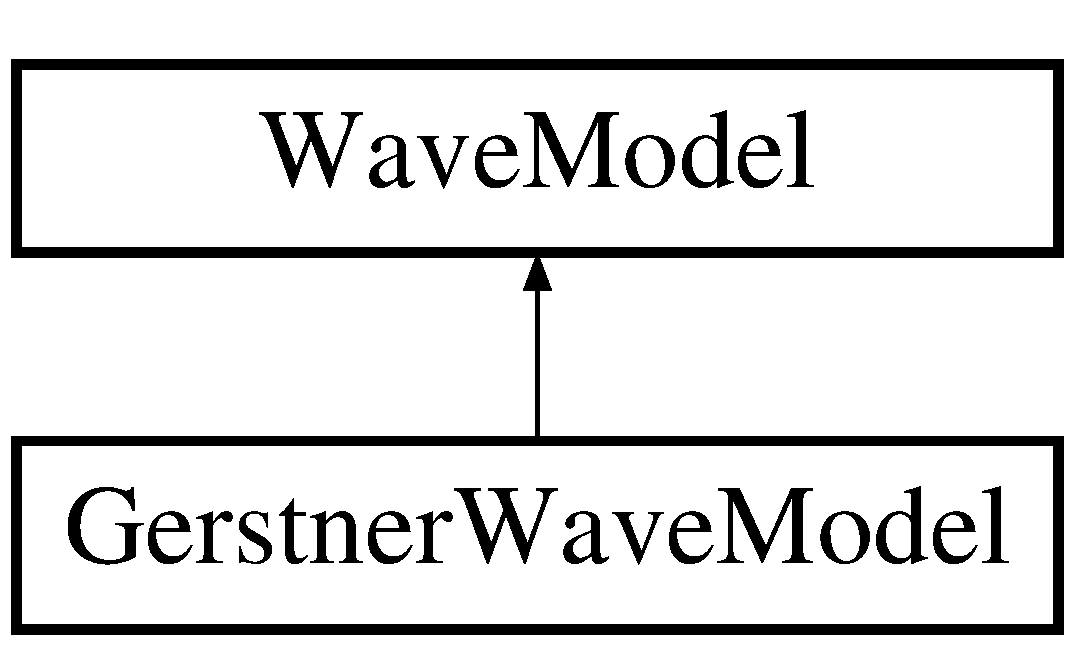
\includegraphics[height=2.000000cm]{class_gerstner_wave_model}
\end{center}
\end{figure}
\subsection*{Public Member Functions}
\begin{DoxyCompactItemize}
\item 
\hypertarget{class_gerstner_wave_model_a4720c379eb0456649f8e4f0112baeee0}{}\label{class_gerstner_wave_model_a4720c379eb0456649f8e4f0112baeee0} 
{\bfseries Gerstner\+Wave\+Model} (double dirX, double dirY=0, double align\+Vague\+Vent=0, double intensite=0, double l\+Onde\+Moy=0, double ajust\+Haut\+Vague=0, int n=10)
\item 
double \hyperlink{class_gerstner_wave_model_af7df138d591a6fb8e8cbda16e26336ab}{operator()} (int x, int y, int t)
\begin{DoxyCompactList}\small\item\em Foncteur. \end{DoxyCompactList}\end{DoxyCompactItemize}
\subsection*{Public Attributes}
\begin{DoxyCompactItemize}
\item 
std\+::vector$<$ \hyperlink{class_gerstner_wave}{Gerstner\+Wave} $>$ \hyperlink{class_gerstner_wave_model_a25b41754840bd8f3aa2691a388ce42c5}{liste\+Gerstner\+Wave}
\end{DoxyCompactItemize}


\subsection{Detailed Description}
Modèle de Gerstner. 

Contient une liste d\textquotesingle{}ondes de Gerstner dont on fait la somme en chaque point pour trouver la hauteur de la houle 

\subsection{Member Function Documentation}
\hypertarget{class_gerstner_wave_model_af7df138d591a6fb8e8cbda16e26336ab}{}\label{class_gerstner_wave_model_af7df138d591a6fb8e8cbda16e26336ab} 
\index{Gerstner\+Wave\+Model@{Gerstner\+Wave\+Model}!operator()@{operator()}}
\index{operator()@{operator()}!Gerstner\+Wave\+Model@{Gerstner\+Wave\+Model}}
\subsubsection{\texorpdfstring{operator()()}{operator()()}}
{\footnotesize\ttfamily double Gerstner\+Wave\+Model\+::operator() (\begin{DoxyParamCaption}\item[{int}]{x,  }\item[{int}]{y,  }\item[{int}]{t }\end{DoxyParamCaption})\hspace{0.3cm}{\ttfamily [virtual]}}



Foncteur. 

Calcul de la hauteur de l\textquotesingle{}onde en sommant celle de chaque onde de la liste en x,y à t


\begin{DoxyParams}{Parameters}
{\em x} & \+: int -\/ ligne\\
\hline
{\em y} & \+: int -\/ colonne\\
\hline
{\em t} & \+: int -\/ temps \\
\hline
\end{DoxyParams}


Implements \hyperlink{class_wave_model}{Wave\+Model}.



\subsection{Member Data Documentation}
\hypertarget{class_gerstner_wave_model_a25b41754840bd8f3aa2691a388ce42c5}{}\label{class_gerstner_wave_model_a25b41754840bd8f3aa2691a388ce42c5} 
\index{Gerstner\+Wave\+Model@{Gerstner\+Wave\+Model}!liste\+Gerstner\+Wave@{liste\+Gerstner\+Wave}}
\index{liste\+Gerstner\+Wave@{liste\+Gerstner\+Wave}!Gerstner\+Wave\+Model@{Gerstner\+Wave\+Model}}
\subsubsection{\texorpdfstring{liste\+Gerstner\+Wave}{listeGerstnerWave}}
{\footnotesize\ttfamily std\+::vector$<$\hyperlink{class_gerstner_wave}{Gerstner\+Wave}$>$ Gerstner\+Wave\+Model\+::liste\+Gerstner\+Wave}

Liste des ondes 

The documentation for this class was generated from the following files\+:\begin{DoxyCompactItemize}
\item 
Gerstner\+Wave\+Model.\+h\item 
Gerstner\+Wave\+Model.\+cpp\end{DoxyCompactItemize}

\hypertarget{class_height}{}\section{Height Class Reference}
\label{class_height}\index{Height@{Height}}


classe representant un tableau 2D de double  




{\ttfamily \#include $<$Height.\+h$>$}

\subsection*{Public Member Functions}
\begin{DoxyCompactItemize}
\item 
\hyperlink{class_height_ae7df55c82f2a3fbe8e1379c4dd003eef}{Height} (double \+\_\+lx, double \+\_\+ly=1.\+0, int \+\_\+nx=1, int \+\_\+ny=1)
\begin{DoxyCompactList}\small\item\em Constructeur. \end{DoxyCompactList}\item 
\hypertarget{class_height_a5aa949bbcd362e4d59fc9d720cf331c6}{}\label{class_height_a5aa949bbcd362e4d59fc9d720cf331c6} 
{\bfseries Height} (\hyperlink{class_height}{Height} const \&)
\item 
\hypertarget{class_height_a1b1db960b77740c413c482dd243a7172}{}\label{class_height_a1b1db960b77740c413c482dd243a7172} 
\hyperlink{class_height}{Height} \& {\bfseries operator=} (const \hyperlink{class_height}{Height} \&)
\item 
void \hyperlink{class_height_a7df615193a661a7f117a56c716e6189e}{init} (double \+\_\+h)
\begin{DoxyCompactList}\small\item\em Initialisation. \end{DoxyCompactList}\item 
double \hyperlink{class_height_a8d2a8c6f51eae0a1382a1557bad13faf}{operator()} (int i, int j) const
\begin{DoxyCompactList}\small\item\em Foncteur. \end{DoxyCompactList}\item 
\hypertarget{class_height_a8270b4bfbb2d5ef5ea256316dd309dbc}{}\label{class_height_a8270b4bfbb2d5ef5ea256316dd309dbc} 
double \& {\bfseries operator()} (int i, int j)
\item 
\hypertarget{class_height_aaa081f8f3456675762b3d74ded8ea026}{}\label{class_height_aaa081f8f3456675762b3d74ded8ea026} 
double \hyperlink{class_height_aaa081f8f3456675762b3d74ded8ea026}{get\+Lx} (void) const
\begin{DoxyCompactList}\small\item\em Accesseur lx. \end{DoxyCompactList}\item 
\hypertarget{class_height_acd15b8e55b68db36661a07c849ff7be1}{}\label{class_height_acd15b8e55b68db36661a07c849ff7be1} 
double \hyperlink{class_height_acd15b8e55b68db36661a07c849ff7be1}{get\+Ly} (void) const
\begin{DoxyCompactList}\small\item\em Accesseur ly. \end{DoxyCompactList}\item 
\hypertarget{class_height_a44f3f951bdf0dbae9a34b1bb43ad4aa6}{}\label{class_height_a44f3f951bdf0dbae9a34b1bb43ad4aa6} 
int \hyperlink{class_height_a44f3f951bdf0dbae9a34b1bb43ad4aa6}{getnx} (void) const
\begin{DoxyCompactList}\small\item\em Accesseur nx. \end{DoxyCompactList}\item 
\hypertarget{class_height_ab5f469a1458efc563530ebd5321a25f9}{}\label{class_height_ab5f469a1458efc563530ebd5321a25f9} 
int \hyperlink{class_height_ab5f469a1458efc563530ebd5321a25f9}{getny} (void) const
\begin{DoxyCompactList}\small\item\em Accesseur ny. \end{DoxyCompactList}\end{DoxyCompactItemize}


\subsection{Detailed Description}
classe representant un tableau 2D de double 

\subsection{Constructor \& Destructor Documentation}
\hypertarget{class_height_ae7df55c82f2a3fbe8e1379c4dd003eef}{}\label{class_height_ae7df55c82f2a3fbe8e1379c4dd003eef} 
\index{Height@{Height}!Height@{Height}}
\index{Height@{Height}!Height@{Height}}
\subsubsection{\texorpdfstring{Height()}{Height()}}
{\footnotesize\ttfamily Height\+::\+Height (\begin{DoxyParamCaption}\item[{double}]{\+\_\+lx,  }\item[{double}]{\+\_\+ly = {\ttfamily 1.0},  }\item[{int}]{\+\_\+nx = {\ttfamily 1},  }\item[{int}]{\+\_\+ny = {\ttfamily 1} }\end{DoxyParamCaption})}



Constructeur. 


\begin{DoxyParams}{Parameters}
{\em \+\_\+lx} & \+: int -\/ taille\\
\hline
{\em \+\_\+ly} & \+: taille\\
\hline
{\em nx} & \+: int -\/ nb discrétisation en x\\
\hline
{\em ny} & \+: int -\/ nb discretisation en y \\
\hline
\end{DoxyParams}


\subsection{Member Function Documentation}
\hypertarget{class_height_a7df615193a661a7f117a56c716e6189e}{}\label{class_height_a7df615193a661a7f117a56c716e6189e} 
\index{Height@{Height}!init@{init}}
\index{init@{init}!Height@{Height}}
\subsubsection{\texorpdfstring{init()}{init()}}
{\footnotesize\ttfamily void Height\+::init (\begin{DoxyParamCaption}\item[{double}]{\+\_\+h }\end{DoxyParamCaption})}



Initialisation. 

Met tous les éléments du tableau à \+\_\+h


\begin{DoxyParams}{Parameters}
{\em \+\_\+h} & \+: double -\/ valeur d\textquotesingle{}initialisation \\
\hline
\end{DoxyParams}
\hypertarget{class_height_a8d2a8c6f51eae0a1382a1557bad13faf}{}\label{class_height_a8d2a8c6f51eae0a1382a1557bad13faf} 
\index{Height@{Height}!operator()@{operator()}}
\index{operator()@{operator()}!Height@{Height}}
\subsubsection{\texorpdfstring{operator()()}{operator()()}}
{\footnotesize\ttfamily double Height\+::operator() (\begin{DoxyParamCaption}\item[{int}]{i,  }\item[{int}]{j }\end{DoxyParamCaption}) const}



Foncteur. 

Accès à l\textquotesingle{}élément (i,j) (indice \+: i$\ast$ny + j) en rvalue


\begin{DoxyParams}{Parameters}
{\em i} & \+: int -\/ ligne\\
\hline
{\em j} & \+: int -\/ colonne \\
\hline
\end{DoxyParams}


The documentation for this class was generated from the following files\+:\begin{DoxyCompactItemize}
\item 
Height.\+h\item 
Height.\+cpp\end{DoxyCompactItemize}

\hypertarget{class_ocean}{}\section{Ocean Class Reference}
\label{class_ocean}\index{Ocean@{Ocean}}


classe faisant la synthèse de toutes les données -\/ calculs des hauteurs  




{\ttfamily \#include $<$Ocean.\+h$>$}

\subsection*{Public Member Functions}
\begin{DoxyCompactItemize}
\item 
\hyperlink{class_ocean_a6a56fee065163c5bd6e5286879648407}{Ocean} (double \+\_\+lx, double \+\_\+ly, int \+\_\+nx, int \+\_\+ny, \hyperlink{class_wave_model}{Wave\+Model} $\ast$\+\_\+model)
\begin{DoxyCompactList}\small\item\em Constructeur. \end{DoxyCompactList}\item 
\hypertarget{class_ocean_af8e1a8ac9f96ae135974e0ed95c61ff8}{}\label{class_ocean_af8e1a8ac9f96ae135974e0ed95c61ff8} 
\hyperlink{class_ocean}{Ocean} \& {\bfseries operator=} (const \hyperlink{class_ocean}{Ocean} \&)
\item 
void \hyperlink{class_ocean_a3f3c62c66d2e25ee9c1fb571f66809e4}{generate\+Height} (double h)
\begin{DoxyCompactList}\small\item\em Initialisation. \end{DoxyCompactList}\item 
void \hyperlink{class_ocean_ae2b45ea776fbb72552af532b2cd8b120}{main\+\_\+computation} (int t)
\begin{DoxyCompactList}\small\item\em Calcul. \end{DoxyCompactList}\item 
\hypertarget{class_ocean_abd4079afe50333f62d206cf1f4ad94b2}{}\label{class_ocean_abd4079afe50333f62d206cf1f4ad94b2} 
int {\bfseries get\+Nx} ()
\item 
\hypertarget{class_ocean_a5d5ec3b226e48b36ea4f0935bab59d90}{}\label{class_ocean_a5d5ec3b226e48b36ea4f0935bab59d90} 
int {\bfseries get\+Ny} ()
\item 
\hypertarget{class_ocean_a7a70306563f904db9d1e45341b0ee17b}{}\label{class_ocean_a7a70306563f904db9d1e45341b0ee17b} 
double {\bfseries get\+\_\+lx} ()
\item 
\hypertarget{class_ocean_abe5c5b3d24ed7521b351e2be630623db}{}\label{class_ocean_abe5c5b3d24ed7521b351e2be630623db} 
double {\bfseries get\+\_\+ly} ()
\item 
void \hyperlink{class_ocean_ad10379d1f92b154eca3936860c96b4f4}{init\+\_\+gl\+\_\+\+Vertex\+ArrayX} (const int y, double $\ast$const vertices) const
\item 
void \hyperlink{class_ocean_a1adbab4eeb806026aff3fb730ca3fe5c}{init\+\_\+gl\+\_\+\+Vertex\+ArrayY} (const int x, double $\ast$const vertices) const
\item 
void \hyperlink{class_ocean_abd9dcb14e3ec076a8623099c0445dc5c}{gl\+\_\+\+Vertex\+ArrayX} (const int y, double $\ast$const vertices) const
\item 
void \hyperlink{class_ocean_a1100e965070ccb68a8f0bec5d5b60a5c}{gl\+\_\+\+Vertex\+ArrayY} (const int x, double $\ast$const vertices) const
\end{DoxyCompactItemize}


\subsection{Detailed Description}
classe faisant la synthèse de toutes les données -\/ calculs des hauteurs 

\subsection{Constructor \& Destructor Documentation}
\hypertarget{class_ocean_a6a56fee065163c5bd6e5286879648407}{}\label{class_ocean_a6a56fee065163c5bd6e5286879648407} 
\index{Ocean@{Ocean}!Ocean@{Ocean}}
\index{Ocean@{Ocean}!Ocean@{Ocean}}
\subsubsection{\texorpdfstring{Ocean()}{Ocean()}}
{\footnotesize\ttfamily Ocean\+::\+Ocean (\begin{DoxyParamCaption}\item[{double}]{\+\_\+lx,  }\item[{double}]{\+\_\+ly,  }\item[{int}]{\+\_\+nx,  }\item[{int}]{\+\_\+ny,  }\item[{\hyperlink{class_wave_model}{Wave\+Model} $\ast$}]{\+\_\+model }\end{DoxyParamCaption})}



Constructeur. 


\begin{DoxyParams}{Parameters}
{\em \+\_\+lx} & \+: int -\/ taille\\
\hline
{\em \+\_\+ly} & \+: taille\\
\hline
{\em nx} & \+: int -\/ nb discrétisation en x\\
\hline
{\em ny} & \+: int -\/ nb discretisation en y\\
\hline
{\em \+\_\+model} & \+: \hyperlink{class_wave_model}{Wave\+Model} -\/ modèle de calcul de houle choisi \\
\hline
\end{DoxyParams}


\subsection{Member Function Documentation}
\hypertarget{class_ocean_a3f3c62c66d2e25ee9c1fb571f66809e4}{}\label{class_ocean_a3f3c62c66d2e25ee9c1fb571f66809e4} 
\index{Ocean@{Ocean}!generate\+Height@{generate\+Height}}
\index{generate\+Height@{generate\+Height}!Ocean@{Ocean}}
\subsubsection{\texorpdfstring{generate\+Height()}{generateHeight()}}
{\footnotesize\ttfamily void Ocean\+::generate\+Height (\begin{DoxyParamCaption}\item[{double}]{h }\end{DoxyParamCaption})}



Initialisation. 


\begin{DoxyParams}{Parameters}
{\em h} & \+: double -\/ création et initialisation du tableau des hauteurs \\
\hline
\end{DoxyParams}
\hypertarget{class_ocean_abd9dcb14e3ec076a8623099c0445dc5c}{}\label{class_ocean_abd9dcb14e3ec076a8623099c0445dc5c} 
\index{Ocean@{Ocean}!gl\+\_\+\+Vertex\+ArrayX@{gl\+\_\+\+Vertex\+ArrayX}}
\index{gl\+\_\+\+Vertex\+ArrayX@{gl\+\_\+\+Vertex\+ArrayX}!Ocean@{Ocean}}
\subsubsection{\texorpdfstring{gl\+\_\+\+Vertex\+Array\+X()}{gl\_VertexArrayX()}}
{\footnotesize\ttfamily void Ocean\+::gl\+\_\+\+Vertex\+ArrayX (\begin{DoxyParamCaption}\item[{const int}]{y,  }\item[{double $\ast$const}]{vertices }\end{DoxyParamCaption}) const}

Convertit le champs de hauteur en tabeau directement utilisable par Open\+GL pour un y donné param\mbox{[}in\mbox{]} y abscisse de la colonne à parcourir param\mbox{[}out\mbox{]} vertices buffer contenant les valeurs aux noeuds \hypertarget{class_ocean_a1100e965070ccb68a8f0bec5d5b60a5c}{}\label{class_ocean_a1100e965070ccb68a8f0bec5d5b60a5c} 
\index{Ocean@{Ocean}!gl\+\_\+\+Vertex\+ArrayY@{gl\+\_\+\+Vertex\+ArrayY}}
\index{gl\+\_\+\+Vertex\+ArrayY@{gl\+\_\+\+Vertex\+ArrayY}!Ocean@{Ocean}}
\subsubsection{\texorpdfstring{gl\+\_\+\+Vertex\+Array\+Y()}{gl\_VertexArrayY()}}
{\footnotesize\ttfamily void Ocean\+::gl\+\_\+\+Vertex\+ArrayY (\begin{DoxyParamCaption}\item[{const int}]{x,  }\item[{double $\ast$const}]{vertices }\end{DoxyParamCaption}) const}

Convertit le champs de hauteur en tabeau directement utilisable par Open\+GL pour un x donné param\mbox{[}in\mbox{]} x abscisse de la ligne à parcourir param\mbox{[}out\mbox{]} vertices buffer contenant les valeurs aux noeuds \hypertarget{class_ocean_ad10379d1f92b154eca3936860c96b4f4}{}\label{class_ocean_ad10379d1f92b154eca3936860c96b4f4} 
\index{Ocean@{Ocean}!init\+\_\+gl\+\_\+\+Vertex\+ArrayX@{init\+\_\+gl\+\_\+\+Vertex\+ArrayX}}
\index{init\+\_\+gl\+\_\+\+Vertex\+ArrayX@{init\+\_\+gl\+\_\+\+Vertex\+ArrayX}!Ocean@{Ocean}}
\subsubsection{\texorpdfstring{init\+\_\+gl\+\_\+\+Vertex\+Array\+X()}{init\_gl\_VertexArrayX()}}
{\footnotesize\ttfamily void Ocean\+::init\+\_\+gl\+\_\+\+Vertex\+ArrayX (\begin{DoxyParamCaption}\item[{const int}]{y,  }\item[{double $\ast$const}]{vertices }\end{DoxyParamCaption}) const}

Initialise la grille dans la direction x param\mbox{[}in\mbox{]} y abscisse de la colonne à parcourir param\mbox{[}out\mbox{]} vertices buffer contenant les coordonnées des noeuds \hypertarget{class_ocean_a1adbab4eeb806026aff3fb730ca3fe5c}{}\label{class_ocean_a1adbab4eeb806026aff3fb730ca3fe5c} 
\index{Ocean@{Ocean}!init\+\_\+gl\+\_\+\+Vertex\+ArrayY@{init\+\_\+gl\+\_\+\+Vertex\+ArrayY}}
\index{init\+\_\+gl\+\_\+\+Vertex\+ArrayY@{init\+\_\+gl\+\_\+\+Vertex\+ArrayY}!Ocean@{Ocean}}
\subsubsection{\texorpdfstring{init\+\_\+gl\+\_\+\+Vertex\+Array\+Y()}{init\_gl\_VertexArrayY()}}
{\footnotesize\ttfamily void Ocean\+::init\+\_\+gl\+\_\+\+Vertex\+ArrayY (\begin{DoxyParamCaption}\item[{const int}]{x,  }\item[{double $\ast$const}]{vertices }\end{DoxyParamCaption}) const}

Initialise la grille dans la direction y param\mbox{[}in\mbox{]} x abscisse de la ligne à parcourir param\mbox{[}out\mbox{]} vertices buffer contenant les coordonnées des noeuds \hypertarget{class_ocean_ae2b45ea776fbb72552af532b2cd8b120}{}\label{class_ocean_ae2b45ea776fbb72552af532b2cd8b120} 
\index{Ocean@{Ocean}!main\+\_\+computation@{main\+\_\+computation}}
\index{main\+\_\+computation@{main\+\_\+computation}!Ocean@{Ocean}}
\subsubsection{\texorpdfstring{main\+\_\+computation()}{main\_computation()}}
{\footnotesize\ttfamily void Ocean\+::main\+\_\+computation (\begin{DoxyParamCaption}\item[{int}]{t }\end{DoxyParamCaption})}



Calcul. 

Calcul du tableau des hauteurs de houle au temps t


\begin{DoxyParams}{Parameters}
{\em t} & \+: int -\/ temps \\
\hline
\end{DoxyParams}


The documentation for this class was generated from the following files\+:\begin{DoxyCompactItemize}
\item 
Ocean.\+h\item 
Ocean.\+cpp\end{DoxyCompactItemize}

\hypertarget{class_philips_wave_model}{}\section{Philips\+Wave\+Model Class Reference}
\label{class_philips_wave_model}\index{Philips\+Wave\+Model@{Philips\+Wave\+Model}}
Inheritance diagram for Philips\+Wave\+Model\+:\begin{figure}[H]
\begin{center}
\leavevmode
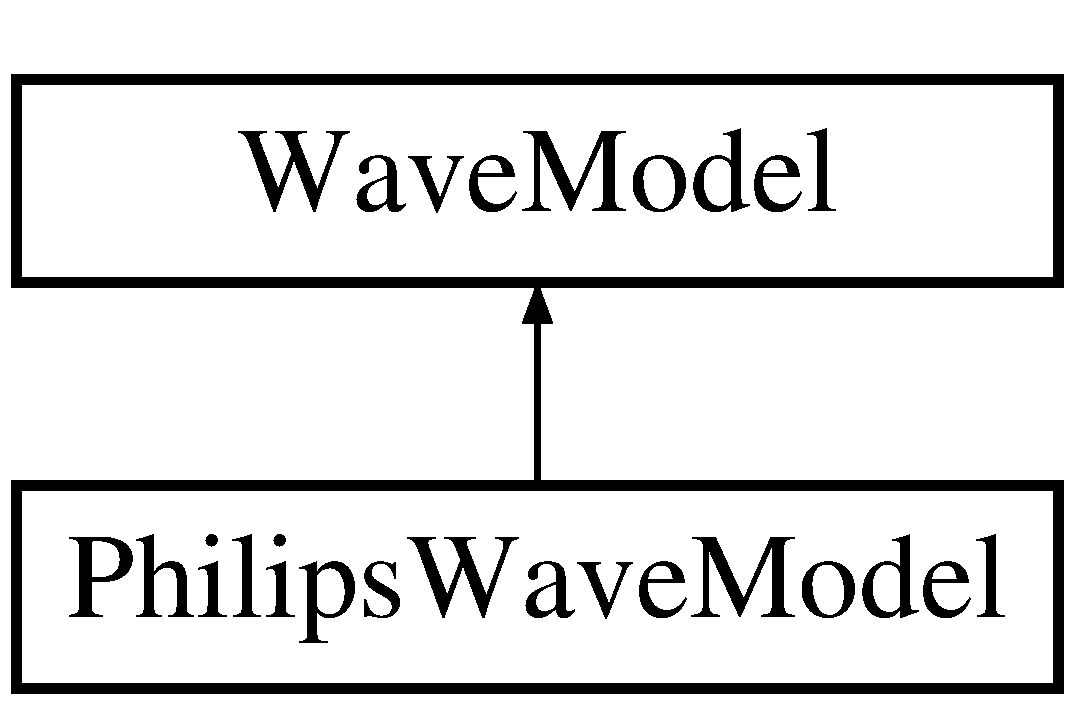
\includegraphics[height=2.000000cm]{class_philips_wave_model}
\end{center}
\end{figure}
\subsection*{Public Member Functions}
\begin{DoxyCompactItemize}
\item 
\hyperlink{class_philips_wave_model_af74356970392e267473590564dfaa4f2}{Philips\+Wave\+Model} (double dirX, double dirY, double align\+Vague\+Vent, double intensite, double l\+Onde\+Moy, double ajust\+Haut\+Vague, int \+\_\+lx, int \+\_\+ly, int \+\_\+nx, int \+\_\+ny)
\begin{DoxyCompactList}\small\item\em Constructeur. \end{DoxyCompactList}\item 
void \hyperlink{class_philips_wave_model_acbd7477d35df750bcd83d8c680eabb83}{init} ()
\begin{DoxyCompactList}\small\item\em Initialisation. \end{DoxyCompactList}\item 
double \hyperlink{class_philips_wave_model_aaefa659dbc00e44430e244a03f2f45ec}{operator()} (int x, int y, int t)
\begin{DoxyCompactList}\small\item\em Foncteur. \end{DoxyCompactList}\end{DoxyCompactItemize}
\subsection*{Additional Inherited Members}


\subsection{Constructor \& Destructor Documentation}
\hypertarget{class_philips_wave_model_af74356970392e267473590564dfaa4f2}{}\label{class_philips_wave_model_af74356970392e267473590564dfaa4f2} 
\index{Philips\+Wave\+Model@{Philips\+Wave\+Model}!Philips\+Wave\+Model@{Philips\+Wave\+Model}}
\index{Philips\+Wave\+Model@{Philips\+Wave\+Model}!Philips\+Wave\+Model@{Philips\+Wave\+Model}}
\subsubsection{\texorpdfstring{Philips\+Wave\+Model()}{PhilipsWaveModel()}}
{\footnotesize\ttfamily Philips\+Wave\+Model\+::\+Philips\+Wave\+Model (\begin{DoxyParamCaption}\item[{double}]{dirX,  }\item[{double}]{dirY,  }\item[{double}]{align\+Vague\+Vent,  }\item[{double}]{intensite,  }\item[{double}]{l\+Onde\+Moy,  }\item[{double}]{ajust\+Haut\+Vague,  }\item[{int}]{\+\_\+lx,  }\item[{int}]{\+\_\+ly,  }\item[{int}]{\+\_\+nx,  }\item[{int}]{\+\_\+ny }\end{DoxyParamCaption})}



Constructeur. 


\begin{DoxyParams}{Parameters}
{\em dirX} & \+: direction du vent selon X\\
\hline
{\em dirY} & \+: direction du vent selon Y\\
\hline
{\em align\+Vague\+Vent} & \+: alignement moyen entre les vagues et le vent\\
\hline
{\em intensite} & \+: intensite du vent\\
\hline
{\em l\+Onde\+Moy} & \+: longueur d\textquotesingle{}onde moyenne des vagues\\
\hline
{\em ajust\+Haut\+Vague} & \\
\hline
\end{DoxyParams}


\subsection{Member Function Documentation}
\hypertarget{class_philips_wave_model_acbd7477d35df750bcd83d8c680eabb83}{}\label{class_philips_wave_model_acbd7477d35df750bcd83d8c680eabb83} 
\index{Philips\+Wave\+Model@{Philips\+Wave\+Model}!init@{init}}
\index{init@{init}!Philips\+Wave\+Model@{Philips\+Wave\+Model}}
\subsubsection{\texorpdfstring{init()}{init()}}
{\footnotesize\ttfamily void Philips\+Wave\+Model\+::init (\begin{DoxyParamCaption}{ }\end{DoxyParamCaption})}



Initialisation. 

Calcul des facteurs de Phillips selon k, ainsi que des fréquences w selon k $<$ norme au carré de k

$<$ norme exposant 4 de k

$<$ fréquence

$<$ Coefficient de Phillips \hypertarget{class_philips_wave_model_aaefa659dbc00e44430e244a03f2f45ec}{}\label{class_philips_wave_model_aaefa659dbc00e44430e244a03f2f45ec} 
\index{Philips\+Wave\+Model@{Philips\+Wave\+Model}!operator()@{operator()}}
\index{operator()@{operator()}!Philips\+Wave\+Model@{Philips\+Wave\+Model}}
\subsubsection{\texorpdfstring{operator()()}{operator()()}}
{\footnotesize\ttfamily double Philips\+Wave\+Model\+::operator() (\begin{DoxyParamCaption}\item[{int}]{x,  }\item[{int}]{y,  }\item[{int}]{t }\end{DoxyParamCaption})\hspace{0.3cm}{\ttfamily [virtual]}}



Foncteur. 

Calcul de la hauteur de l\textquotesingle{}onde en sommant celle de chaque onde de la liste en x,y à t


\begin{DoxyParams}{Parameters}
{\em x} & \+: int -\/ ligne\\
\hline
{\em y} & \+: int -\/ colonne\\
\hline
{\em t} & \+: int -\/ temps \\
\hline
\end{DoxyParams}


Implements \hyperlink{class_wave_model}{Wave\+Model}.



The documentation for this class was generated from the following files\+:\begin{DoxyCompactItemize}
\item 
Philips\+Wave\+Model.\+h\item 
Philips\+Wave\+Model.\+cpp\end{DoxyCompactItemize}

\hypertarget{class_wave_model}{}\section{Wave\+Model Class Reference}
\label{class_wave_model}\index{Wave\+Model@{Wave\+Model}}
Inheritance diagram for Wave\+Model\+:\begin{figure}[H]
\begin{center}
\leavevmode
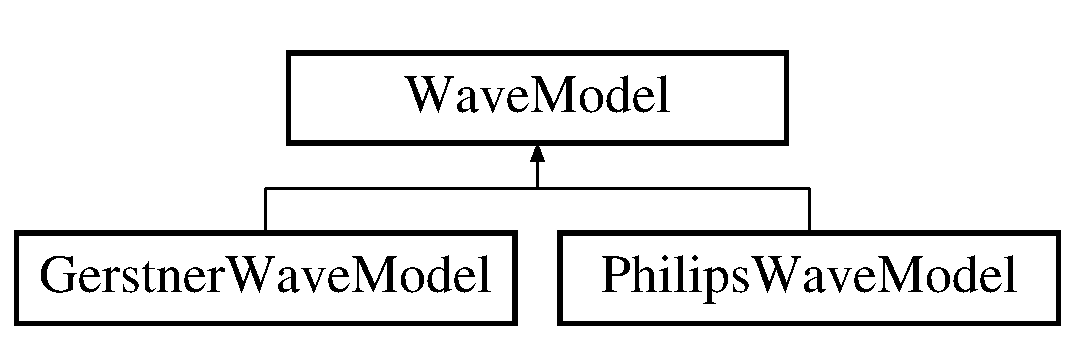
\includegraphics[height=2.000000cm]{class_wave_model}
\end{center}
\end{figure}
\subsection*{Public Member Functions}
\begin{DoxyCompactItemize}
\item 
\hypertarget{class_wave_model_a889a450cd0249533c42481818121cb88}{}\label{class_wave_model_a889a450cd0249533c42481818121cb88} 
virtual double {\bfseries operator()} (int x, int y, int t)=0
\item 
\hypertarget{class_wave_model_a4fe96b7c5d499212f104d576c1623e55}{}\label{class_wave_model_a4fe96b7c5d499212f104d576c1623e55} 
{\bfseries Wave\+Model} (double dirX, double dirY=0, double align\+Vague\+Vent=0, double intensite=0, double l\+Onde\+Moy=0, double ajust\+Haut\+Vague=0)
\item 
\hypertarget{class_wave_model_a25791da686d3d80e605ec2d5119a0a77}{}\label{class_wave_model_a25791da686d3d80e605ec2d5119a0a77} 
{\bfseries Wave\+Model} (\hyperlink{class_wave_model}{Wave\+Model} const \&w)
\item 
\hypertarget{class_wave_model_acbbb099975edc7b7ef03b23deb67bd68}{}\label{class_wave_model_acbbb099975edc7b7ef03b23deb67bd68} 
\hyperlink{class_wave_model}{Wave\+Model} \& {\bfseries operator=} (const \hyperlink{class_wave_model}{Wave\+Model} \&w)
\item 
\hypertarget{class_wave_model_a5ab74b10cb5573a3c2fe6fcb2820e9ba}{}\label{class_wave_model_a5ab74b10cb5573a3c2fe6fcb2820e9ba} 
double {\bfseries get\+DirX} (void) const
\item 
\hypertarget{class_wave_model_aba929e2efa38f19639a645ec085a01d3}{}\label{class_wave_model_aba929e2efa38f19639a645ec085a01d3} 
double {\bfseries get\+DirY} (void) const
\item 
\hypertarget{class_wave_model_a3e04992c8898eed9ad112d273e432787}{}\label{class_wave_model_a3e04992c8898eed9ad112d273e432787} 
double {\bfseries get\+Align\+Vague\+Vent} (void) const
\item 
\hypertarget{class_wave_model_ac93f79a9ccb22f5d57cd7bbe543fa728}{}\label{class_wave_model_ac93f79a9ccb22f5d57cd7bbe543fa728} 
double {\bfseries get\+Intensite} (void) const
\item 
\hypertarget{class_wave_model_a4e9e1d1a5be89413beea6ae8c72adc39}{}\label{class_wave_model_a4e9e1d1a5be89413beea6ae8c72adc39} 
double {\bfseries get\+L\+Onde\+Moy} (void) const
\item 
\hypertarget{class_wave_model_a24d40f4090721841f2e7b1b1a329f2c8}{}\label{class_wave_model_a24d40f4090721841f2e7b1b1a329f2c8} 
double {\bfseries get\+Ajust\+Haut\+Vague} (void) const
\end{DoxyCompactItemize}
\subsection*{Public Attributes}
\begin{DoxyCompactItemize}
\item 
\hypertarget{class_wave_model_ab4822ed59164d1c8316e23452c7bee83}{}\label{class_wave_model_ab4822ed59164d1c8316e23452c7bee83} 
double {\bfseries dirX}
\item 
\hypertarget{class_wave_model_a7fbe1eaf5059ef0b3dba4b0052db5446}{}\label{class_wave_model_a7fbe1eaf5059ef0b3dba4b0052db5446} 
double {\bfseries dirY}
\item 
\hypertarget{class_wave_model_aae60d61d9b0e55999ef05bb5deb5ac04}{}\label{class_wave_model_aae60d61d9b0e55999ef05bb5deb5ac04} 
double {\bfseries align\+Vague\+Vent}
\item 
\hypertarget{class_wave_model_a2bda2f93c3cc1cebcb9d7d3c7c4e52a8}{}\label{class_wave_model_a2bda2f93c3cc1cebcb9d7d3c7c4e52a8} 
double {\bfseries intensite}
\item 
\hypertarget{class_wave_model_ac9f38b5b6a556fd4b1e0d0b97916df05}{}\label{class_wave_model_ac9f38b5b6a556fd4b1e0d0b97916df05} 
double {\bfseries l\+Onde\+Moy}
\item 
\hypertarget{class_wave_model_a2bdc077ae85c1eca6e46fe67936fbf23}{}\label{class_wave_model_a2bdc077ae85c1eca6e46fe67936fbf23} 
double {\bfseries ajust\+Haut\+Vague}
\end{DoxyCompactItemize}


The documentation for this class was generated from the following files\+:\begin{DoxyCompactItemize}
\item 
Wave\+Model.\+h\item 
Wave\+Model.\+cpp\end{DoxyCompactItemize}

\chapter{File Documentation}
\hypertarget{_dvector_8h}{}\section{Dvector.\+h File Reference}
\label{_dvector_8h}\index{Dvector.\+h@{Dvector.\+h}}


Vecteur de base (T\+P1 et T\+P2)  


{\ttfamily \#include $<$iostream$>$}\newline
{\ttfamily \#include $<$fstream$>$}\newline
{\ttfamily \#include $<$string$>$}\newline
{\ttfamily \#include $<$cstdio$>$}\newline
{\ttfamily \#include $<$stdio.\+h$>$}\newline
{\ttfamily \#include $<$stdlib.\+h$>$}\newline
{\ttfamily \#include $<$time.\+h$>$}\newline
{\ttfamily \#include $<$assert.\+h$>$}\newline
\subsection*{Classes}
\begin{DoxyCompactItemize}
\item 
class \hyperlink{class_dvector}{Dvector}
\begin{DoxyCompactList}\small\item\em classe representant un vecteur de double \end{DoxyCompactList}\end{DoxyCompactItemize}
\subsection*{Functions}
\begin{DoxyCompactItemize}
\item 
\hypertarget{_dvector_8h_ac6b80b11756db4d5f66b89ea69c04064}{}\label{_dvector_8h_ac6b80b11756db4d5f66b89ea69c04064} 
\hyperlink{class_dvector}{Dvector} {\bfseries operator+} (const \hyperlink{class_dvector}{Dvector} \&, const double d)
\item 
\hypertarget{_dvector_8h_a74c0937806fd74e8cb3e795674d7caaa}{}\label{_dvector_8h_a74c0937806fd74e8cb3e795674d7caaa} 
\hyperlink{class_dvector}{Dvector} {\bfseries operator-\/} (const \hyperlink{class_dvector}{Dvector} \&, const double d)
\item 
\hypertarget{_dvector_8h_a97a0a3760f9eb1bce487bc87665555b1}{}\label{_dvector_8h_a97a0a3760f9eb1bce487bc87665555b1} 
\hyperlink{class_dvector}{Dvector} {\bfseries operator$\ast$} (const \hyperlink{class_dvector}{Dvector} \&, const double d)
\item 
\hypertarget{_dvector_8h_ac7d35ba58d4e80e8d687978dd31f08d1}{}\label{_dvector_8h_ac7d35ba58d4e80e8d687978dd31f08d1} 
\hyperlink{class_dvector}{Dvector} {\bfseries operator/} (const \hyperlink{class_dvector}{Dvector} \&, const double d)
\item 
\hypertarget{_dvector_8h_a4a0c17d7afe72b60bdd380718b67f235}{}\label{_dvector_8h_a4a0c17d7afe72b60bdd380718b67f235} 
\hyperlink{class_dvector}{Dvector} {\bfseries operator+} (const \hyperlink{class_dvector}{Dvector} \&, const \hyperlink{class_dvector}{Dvector} \&)
\item 
\hypertarget{_dvector_8h_a57597c74af2b343a69a4291e4e225335}{}\label{_dvector_8h_a57597c74af2b343a69a4291e4e225335} 
\hyperlink{class_dvector}{Dvector} {\bfseries operator-\/} (const \hyperlink{class_dvector}{Dvector} \&, const \hyperlink{class_dvector}{Dvector} \&)
\item 
\hypertarget{_dvector_8h_a00717b7ec749da5af3434397b4f78d60}{}\label{_dvector_8h_a00717b7ec749da5af3434397b4f78d60} 
\hyperlink{class_dvector}{Dvector} {\bfseries operator-\/} (const \hyperlink{class_dvector}{Dvector} \&)
\item 
\hypertarget{_dvector_8h_a15a4326239ffec5b094248858487272b}{}\label{_dvector_8h_a15a4326239ffec5b094248858487272b} 
ostream \& {\bfseries operator$<$$<$} (ostream \&Out, const \hyperlink{class_dvector}{Dvector} \&D)
\item 
\hypertarget{_dvector_8h_a96fd6e6012f5981e53d5835895b239c1}{}\label{_dvector_8h_a96fd6e6012f5981e53d5835895b239c1} 
istream \& {\bfseries operator$>$$>$} (istream \&In, const \hyperlink{class_dvector}{Dvector} \&D)
\end{DoxyCompactItemize}


\subsection{Detailed Description}
Vecteur de base (T\+P1 et T\+P2) 

\begin{DoxyAuthor}{Author}
baudetgl-\/romeroq 
\end{DoxyAuthor}

%--- End generated contents ---

% Index
\backmatter
\newpage
\phantomsection
\clearemptydoublepage
\addcontentsline{toc}{chapter}{Index}
\printindex

\end{document}
